\documentclass{report}
\input{preamble}
\input{macros}
\input{letterfonts}
\usepackage{pgfplots}
\usepackage{xcolor}
\usepackage{amsmath}
\title{\Huge{Information Theory}\\University of Cambridge}
\author{\huge{Jasmeet Bhatia}}
\date{}

\begin{document}

\maketitle
\newpage% or \cleardoublepage
% \pdfbookmark[<level>]{<title>}{<dest>}
\pdfbookmark[section]{\contentsname}{toc}
\tableofcontents
\pagebreak

\chapter{Lectures 1 and 2}
\section{Introduction to Information Theory}
\dfn{Shannon's Definition of Information (h)}{Let an ensemble, X, have input ($x, A_x, P_x$) where x is a random variable, $A_x$ is a set of possible outcomes ($a_1,a_2,a_3, ... a_1$) and where $P_x$ is the set of possibilities $P_x = (P_1,P_2, ... P_i)$ such that P(x=$a_i$) = $P_i$, we define Shannon's information content as the following: \[ x = a_i h(x=a_i) = log_2 \] 
\[ \therefore h(x = a_i) = log_2 \frac{1}{P(x=a_i)}  \]}

\section{Shannon Plot of Information}
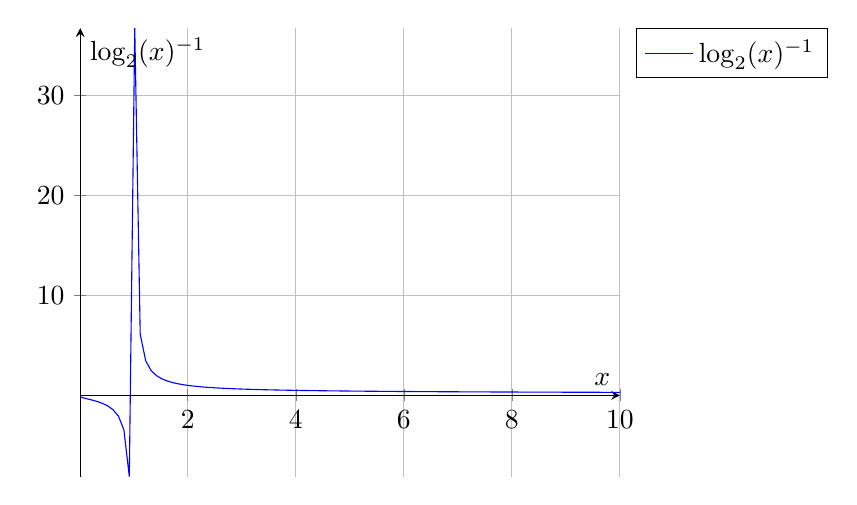
\begin{tikzpicture}
\begin{axis}[
    xlabel=$x$,
    ylabel={$\log_2(x)^{-1}$},
    domain=0.01:10,
    samples=100,
    axis lines=middle,
    grid,
    legend pos=outer north east,
]
\addplot[blue] {1/(ln(x)/ln(2))};
\legend{$\log_2(x)^{-1}$}
\end{axis}
\end{tikzpicture}
\clm{Additive Property}{}{h is additive for independent random variable}

\ex{XY}{$x,y = P(x,y) = P(x)P(y)$ and $x,y.$ Then $h(x,y) = log_2\frac{1}{P(x,y)} = log_2\frac{1}{P(x)} + log_2\frac{1}{P(y)}$. Based on this definition and graph above, we see that the Shannon information thoery shows that the h is largest for outcomes that are the most improbable.}

\section{Entropy H(x)}
\dfn{Entropy H(X)}{Entropy of an ensemble is the average Shannon Information Content (h)
	\[
		H(x) = - \sum P(X)log_2\frac{1}{P(x)}	\]}
		\nt{Entropy H(x) is in units of bits}
		\ex{Applying Entropy to Weighing Ball Problem}{ Comparing 6 Balls against 6 Balls with 12 Balls Total
		\[ H(x) = 0.5log_2\frac{1}{0.5} = 1 bit\]
	Comparing 5 balls against 5 balls with 2 balls on the table
\[H(x) = (1/6)log_2\frac{1}{12/2} + \]
\begin{tabular}{|c|c|c|c|}
\hline
\textbf{} & \textbf{Left Ball is Heavier} & \textbf{Balls is Balanced} & \textbf{Right Ball is Heavier} \\ \hline
Probability & 1/6 & 4/6 & 1/6 \\ \hline
-p * log2(p) & -(1/6) * log2(1/6)  &  -(4/6) * log2(4/6) &  -(1/6) * log2(1/6) \\ \hline
\end{tabular}

Based on this, \[ H(x) = -(1/6)log_2(1/6) -(4/6)log_2(4/6) -(1/6)log_2(1/6) = 1.251 bits \]}
\chapter{Lecture 3}

\clm{Source Coding Theorem}{}{\textcolor{red}{$N$} outcomes from a source \textcolor{red}{$X$} can be compressed into roughly \textcolor{red}{$NH(X)$} bits.}

\ex{Bent Coin Lotter}{A coin with $p_1$ will be tossed $N = 1000$ times. The outcome is x = $x_1,x_2,...x_n$
e.g x = 00000100100...00010
You can buy $2^n$ possible tickers for \$1 each, before the coin-tossing. If you own ticket x, you win \$1,000,000,000.}

\qs{problem}{To have a 99\% chance of winning, at lowest possible cost, which tickets would you buy?
    And how many tickets is that?
Express your answer in the form $2^{(...)}$}


\ex{Sixty-Three}{$x \in \{0,1,2,3,4,5,6 ...,63\}$ \\How can one play the game? One strategy is to split the numbers in half and ask questions that give the most information. \\ $ X\%32 \geq 16? \\ 
X\%16 \geq 8? \\ 
X\%8 \geq 4? $ \\
\[h(c_i) = log_2\frac{1}{P(c_i)}(2) = 1 bit\]
Total Shannon Information Content gained = 6 bits. The string $c_1 ... c_6$ is an encoding of x, defined as c(x) where c(42) - 10100.}
\qs{Generalize}{If there are \textcolor{red}{S} possible outcomes, \textcolor{red}{how many bits long} must each name be, if each outcome has a unique name?
Answer: $\lceil log_2(S) \rceil$ An outcome from a set of size S can be communicated in  $\lceil log_2(S) \rceil$ bits\\\
}

\section{Submarine}
\ex{Submarine}{
    \[
\begin{array}{cccccccc}
0 & 0 & 0 & 0 & 0 & 0 & 0 & 0 \\
0 & 0 & 0 & 0 & 0 & 0 & 0 & 0 \\
0 & 0 & 0 & 0 & 0 & 0 & 0 & 0 \\
0 & 0 & 0 & 0 & 0 & 0 & 0 & 0 \\
0 & 0 & 0 & 0 & 0 & 0 & 0 & 0 \\
0 & 0 & 0 & 1 & 0 & 0 & 0 & 0 \\
0 & 0 & 0 & 0 & 0 & 0 & 0 & 0 \\
0 & 0 & 0 & 0 & 0 & 0 & 0 & 0 \\
\end{array}
\]



\[P(r_1 = n) = \frac{63}{64} \] = 0.0227 bits

\[P(r_1 = n) = \frac{63}{64} \] = 0.0227 bits
}
\section{Bent Coin Lottery}
\ex{Bent Coin Lottery}{A coin with $p_1$ will be tossed N = 1000 times. The outcome is x = $x_1,x_2, ... x_N$. e.g. x = 000001001000100...00010
    You can buy any of the $2^N$ possible tickets for \$1 each, before the coin tossing. If you own ticket x, you win \$1,000,000,000.
    \qs{1}{If you are forced to buy one ticket, which would you buy?
    The all zeroes ticket has the highest chance}
    \qs{}{To have a 99\% chance of winning at lowest possible cost, which tickets would you buy? And how many tickets is that? Express your answer in the form $2^{(...)}$
    } Number of tickets (in order to acquire 99\% probability to win) = $1 + 1000 + \binom{1000}{2} + ... + \binom{1000}{101} + \binom{1000}{102} +  ... + \binom{1000}{122} + \binom{1000}{123}$
}
\chapter{Lecture 4}
\section{File Compression}

\clm{Source Coding Theorem}{}{\textcolor{red}{$N$} outcomes from a source \textcolor{red}{$X$} can be compressed into roughly \textcolor{red}{$NH(X)$} bits.}

Proved by counting \textcolor{red}{the typical set}
When a source \textcolor{red}{X} produces \textcolor{red}{N} indpendent outcomes

\textcolor{red}{$x = x_1x_2 ... x_N$}
this string is very likely to be one of the \textcolor{red}{$~2^{NH(X)}$} \textcolor{green}{typical} outcomes all of which have probability \textcolor{red}{$~2^{-NH(X)}$} 



\end{document}
